%%%%%%%%%%%%----------------------------------------------------------------------------------%%%%%%%%%%%%%%%
\section{GroupTesting}
\subsection{Main result}
\begin{frame}\frametitle{Group Testing}
	\begin{figure}[t]
		\centering
		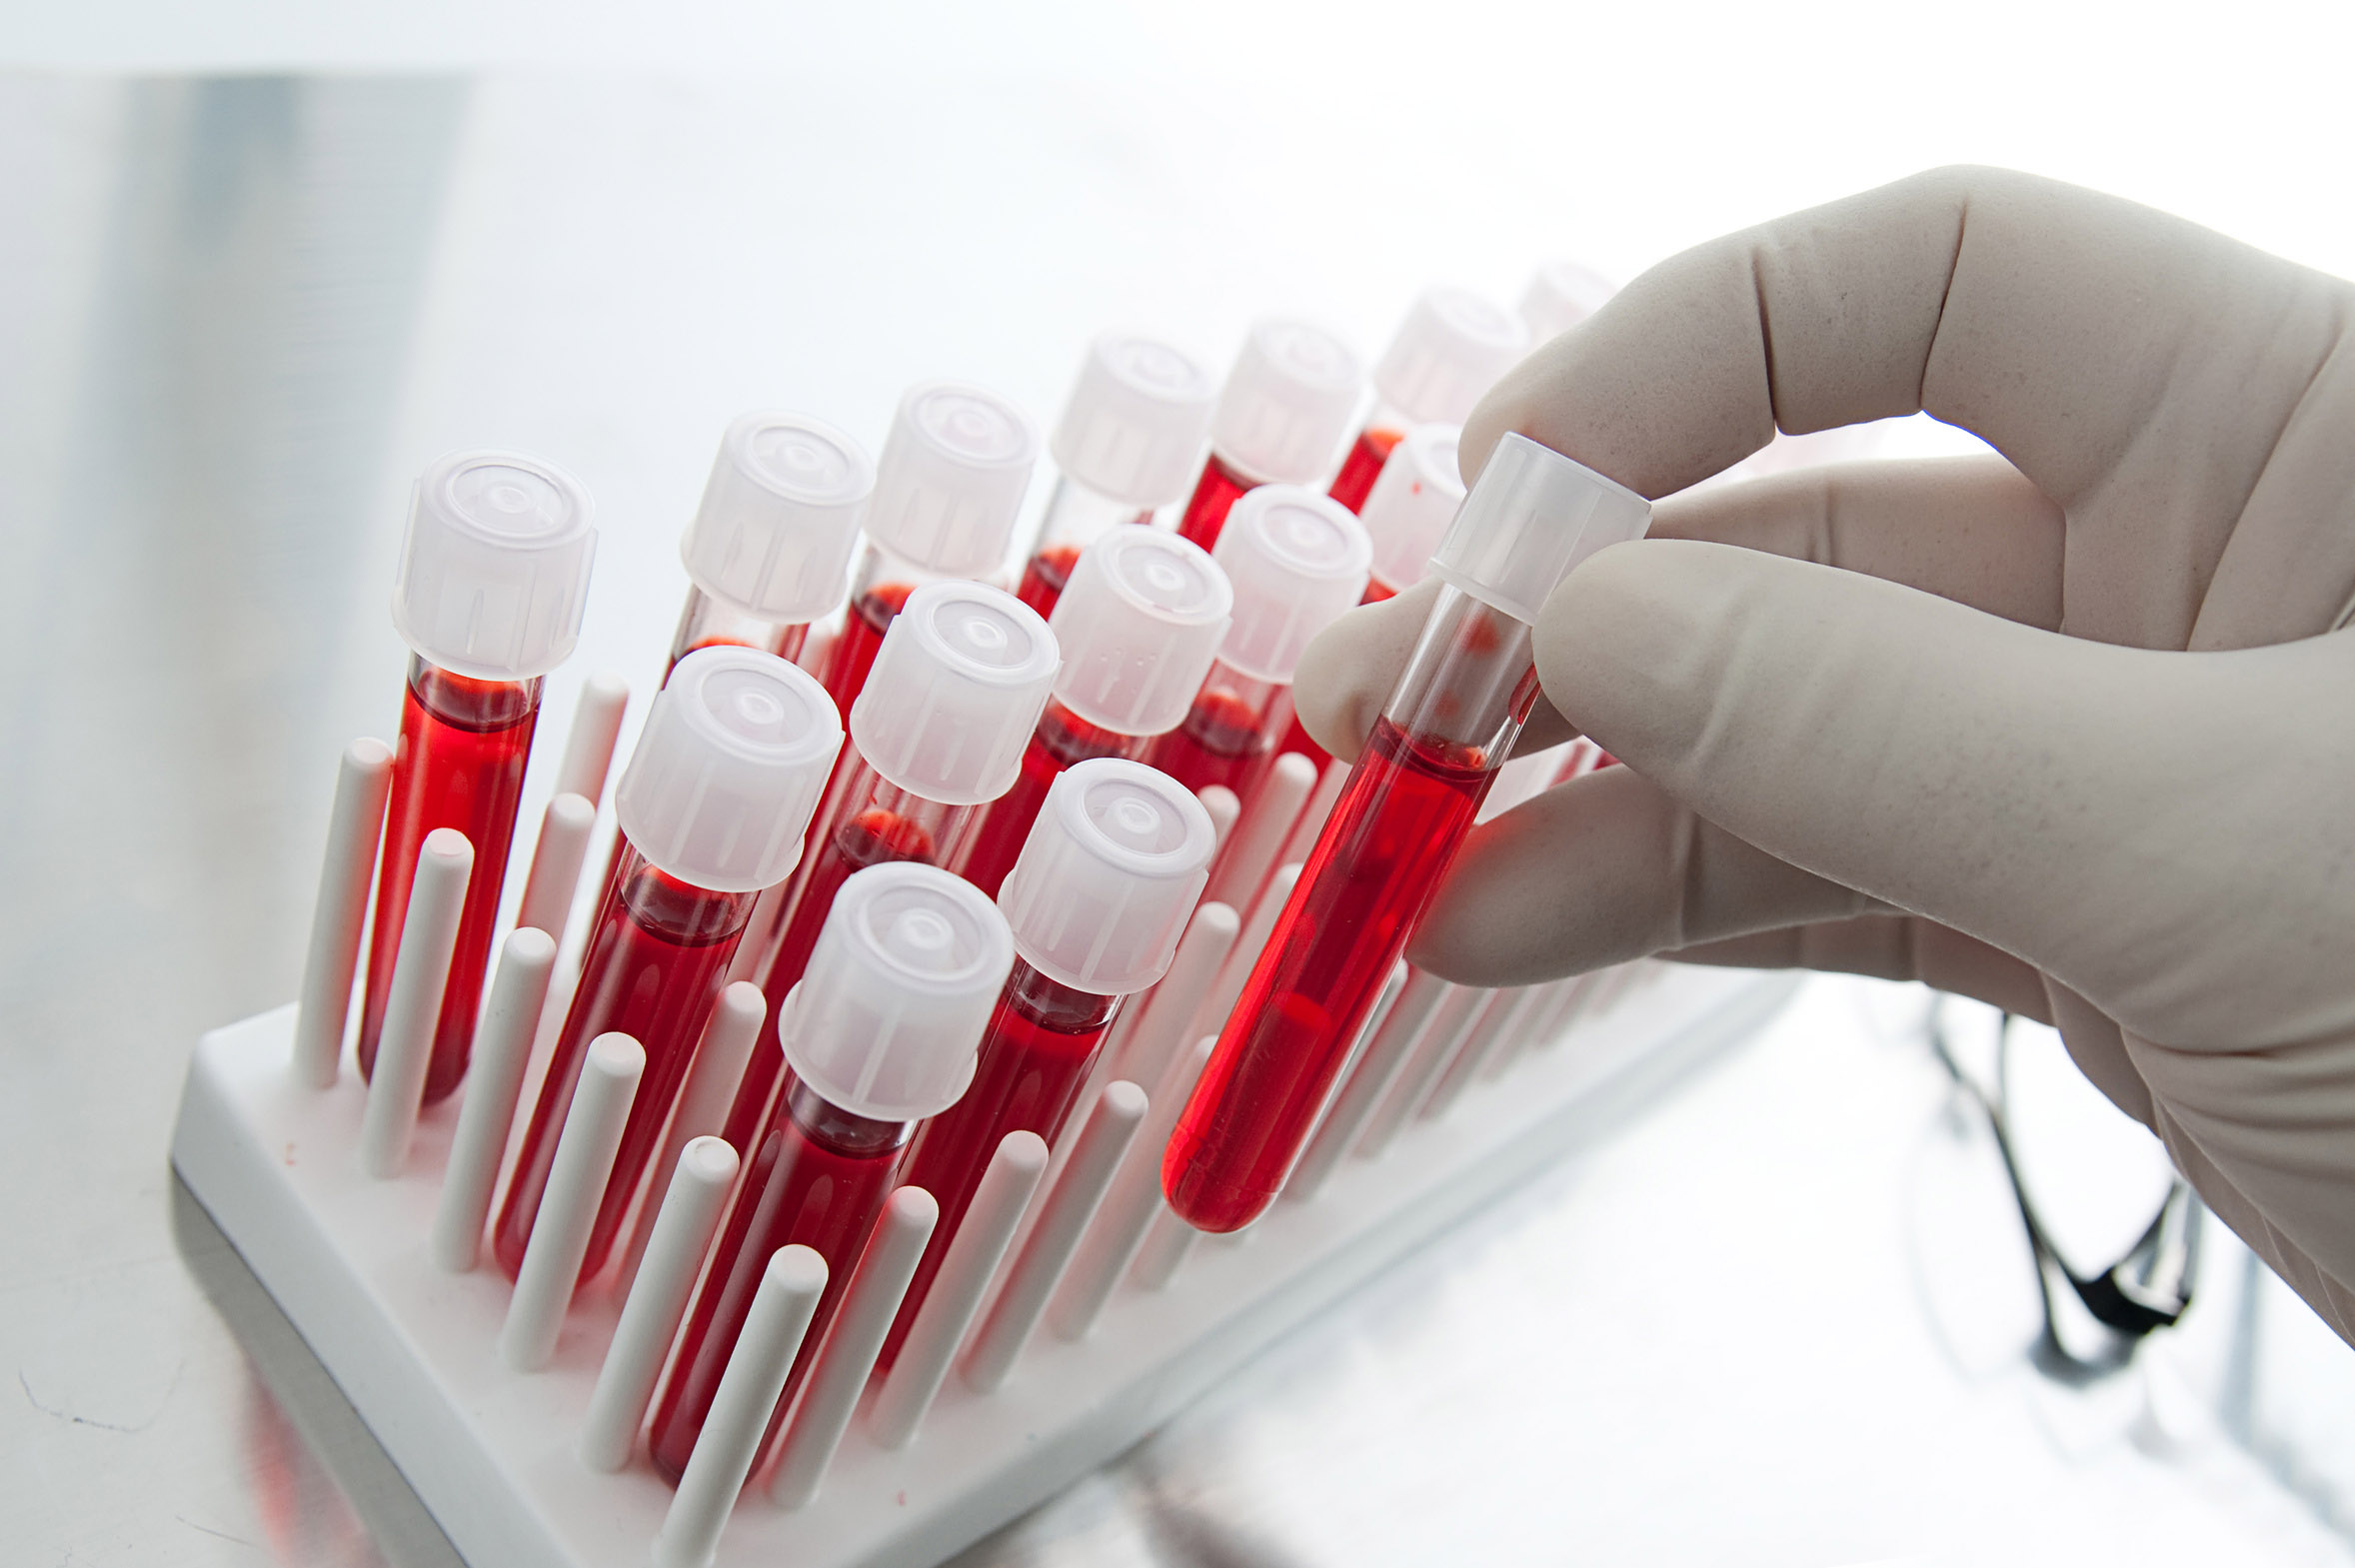
\includegraphics[width=1.8in]{\gt_figpath/grouptest_testubes.jpg}
	\end{figure}

\begin{itemize}
	\item World War II - detect all soldiers with syphilis
	\item Tests performed on efficiently pooled groups of soldiers
	\pause
	\item \emph{Generalized}: Least no. of tests to identify $K$ defective items from $N$ items
\end{itemize}	

\end{frame}

%%%------------------------------------------------------------------------------------------------------------------------------------------
\begin{frame}\frametitle{Introduction}
Example:
\vspace{-0.3in}
	\begin{figure}[t]
		\centering
		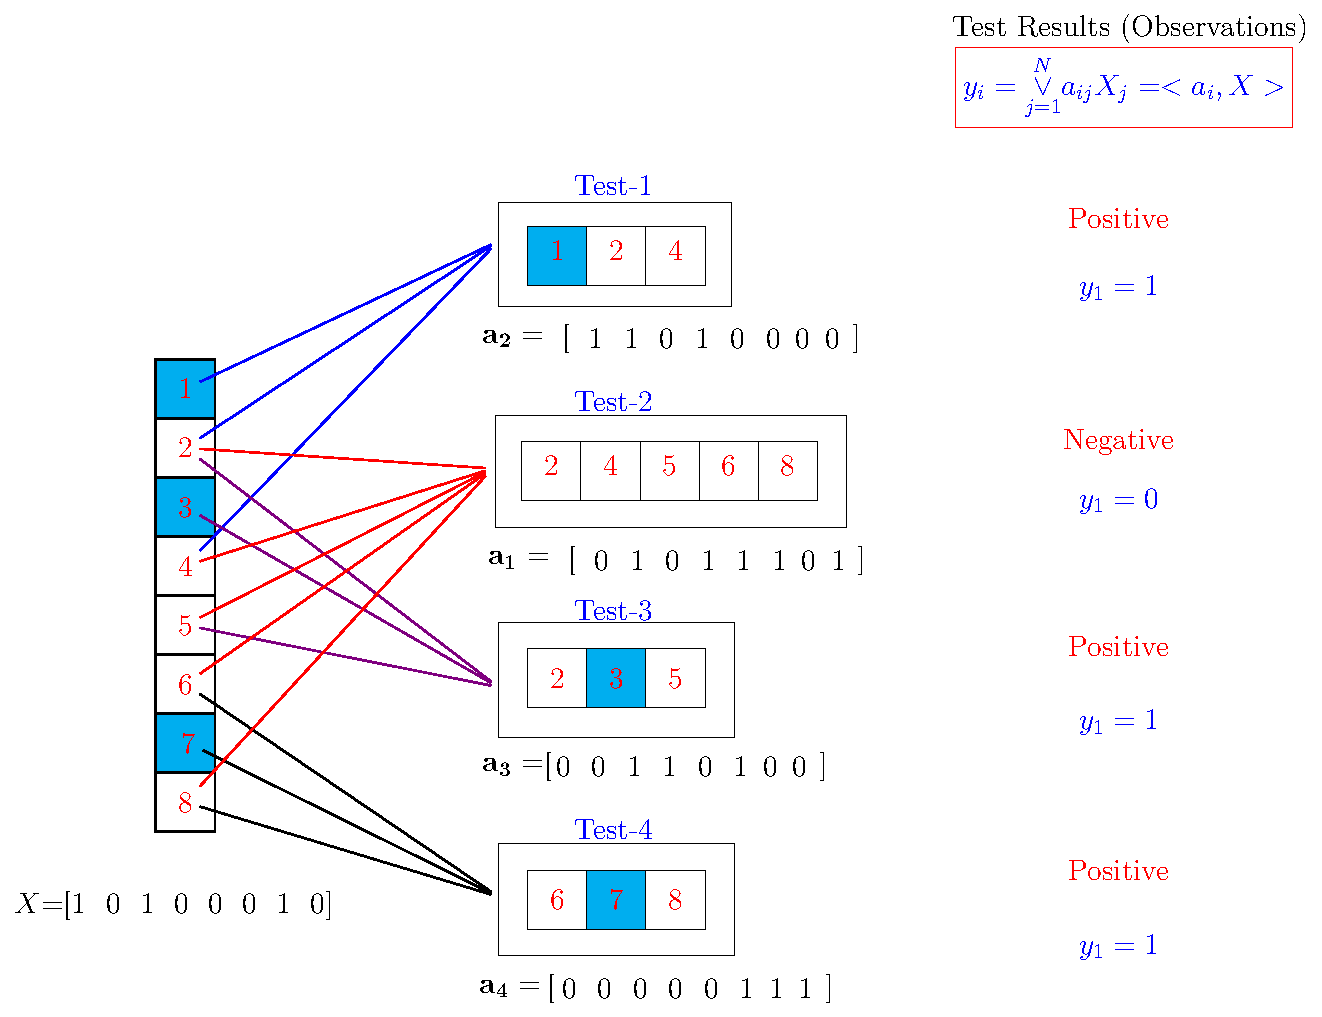
\includegraphics[width=4.2in]{\gt_figpath/grouptesting_example.pdf}
	\end{figure}
\end{frame}

%%---------------------------------------------------------------------------------------------------------------------------------------------
\begin{frame} \frametitle{Problem statement}
\centering
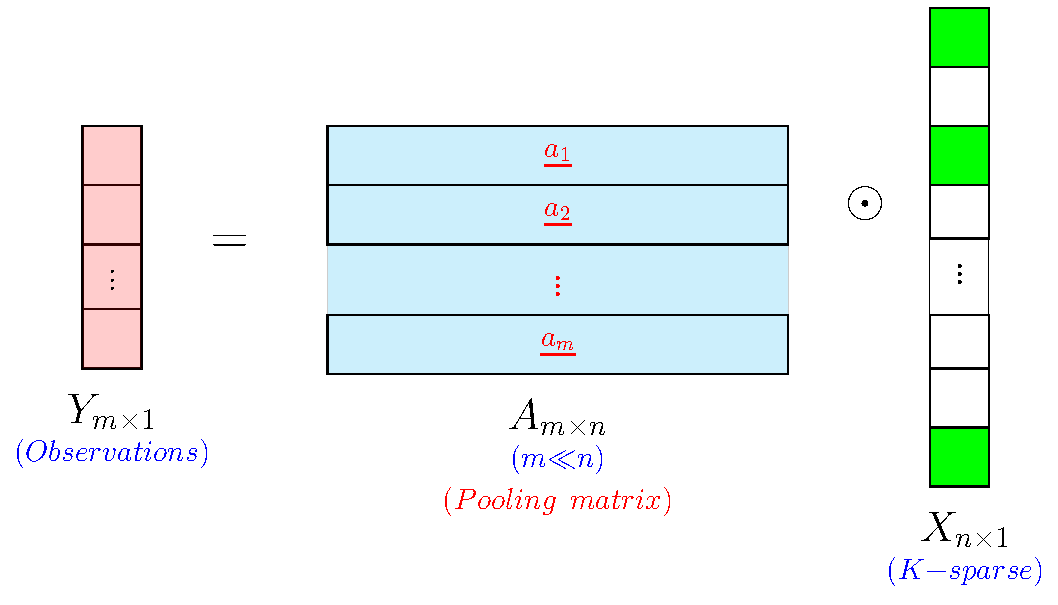
\includegraphics[width=0.58\textwidth]{\gt_figpath/A_times_X_group_testing.pdf}
\[
~~\text{ where~~}		\vec{a}_i\odot X ~= \overset{N}{\underset{j=1}{\vee}} a_{ij}X_j 
\]
\pause
\begin{block}{Objective}
For a given $K,N$ and a maximum probability of recovery error, design a testing scheme
\begin{itemize}
\item minimizing the number of tests
\item minimizing the computational complexity of recovery 
\end{itemize} 
\end{block}
\end{frame}
%%%----------------------------------------------------------------------------------------------------------------------------------
\begin{frame} \frametitle{Bounds on sample and time complexities}
\begin{block}{Probabilistic GT}
\begin{itemize}
\item aim is to recover \emph{all} the defective items w.h.p
\item testing complexity $m$ is $\Omega(K\log \frac{N}{K})$ and $\mc{O}(K\frac{\log^2 N}{\log K})$
\end{itemize}
\end{block}

\pause
\vspace{6ex}
\begin{block}{Approximate GT}
\begin{itemize}
\item aim is to recover ($1-\epsilon$) fraction of the defective items w.h.p
\item testing complexity $m$ is $\mc{O}(K\log N)$
\item lower bound not known
\end{itemize}
\end{block}

\end{frame}

%----------------------------------------------------------------------------------------------------------------------------------
\begin{frame} \frametitle{Main result}
\begin{itemize}
\item We propose a testing scheme based on left and right regular Tanner graphs
\item Bin detection matrix and peeling decoder identical to [LPR 15]
\end{itemize}

\begin{block}{Approximate Group Testing (Noiseless and Noisy)}
\begin{itemize}
\item Recovers $(1-\epsilon)K$ items w.h.p.
\item Samples: $m = c_{\epsilon}K \log_2 \frac{N}{K}$ is order optimal
\begin{itemize}
\item scaling $\mc{O}(K \log N)$ is same as [LPR15]
\item however our scheme provides a better upper bound $\Theta(K\log\frac{N}{K})$
\end{itemize}
\end{itemize}
\end{block}

\pause
\begin{block}{Probabilistic Group Testing}
\begin{itemize}
\item Recovers $K$ defective items w.h.p.
\item With $m = cK \log K \log_2 \frac{N}{K}$ tests, probability of recovery $1-\mc{O}(K^{-\alpha})$
\begin{itemize}
\item only a factor of $\log K$ away from the lower bound $\Omega(K\log\frac{N}{K})$
\end{itemize}
\end{itemize}
\end{block}

\begin{itemize}
\item<3-> Computational complexity: $O(K \log \frac{N}{K})$
\end{itemize}
\end{frame}

%%%-----------------------------------------------------------------------------------------
\subsection{Testing scheme}
\begin{frame}{Challenges to a peeling approach}
\begin{itemize}
\item Differs from CS: OR operation instead of real/binary sum
\item Challenges involved with peeling approach:
\begin{itemize}
\item non-linear function node
\item peeling is difficult. Given $\vec{y}_j=\vec{s}_{1}\vee \vec{s}_{2}\vee \ldots \vec{s}_{k}$ and $\{\vec{s}_1,\ldots \vec{s}_{k-1}\}$, find $\vec{s}_k$? 
\end{itemize}
\end{itemize}
\vspace{3ex}
\pause

\begin{block}{Idea [LPR15]}
Design the bin detection matrix $\mathbf{S}$ such that, given
\begin{itemize}
\item  $\vec{y}_j=\vec{s}_{i_1}$ find $i_1$ efficiently
\item $\vec{y}_j=\vec{s}_{i_1}\vee \vec{s}_{i_2}$ and $i_1$ is known find $i_2$
\item<3-> Peeling decoder involving function nodes with not more than two connections
\end{itemize}

\end{block}
\end{frame}

%%%---------------------------------------------------------------------------------
\begin{frame}\frametitle{Bin detection matrix}
\begin{align*}
{
\small
\mathbf{S}=\begin{bmatrix}
					\bf{b_1} & \bf{b_2} & \bf{b_3} & \cdots & \bf{b_{n-1}}\\
					\vspace{0.2pt}
				   	\bf{\overline{b}_1} & \bf{\overline{b}_2} & \bf{\overline{b}_3} & \cdots & \bf{\overline{b}_{n-1}} \end{bmatrix}
=
 \begin{bmatrix}
		0      & 0   & 0 & \cdots & 1 &  1 \\
		0      & 0   & 0 & \cdots & 1 &  1  \\
		\vdots & \vdots & \vdots & \ddots & \vdots & \vdots \\
		0      & 0   & 1 & \cdots & 1 &  1  \\
		0      & 1   & 0 & \cdots & 0 &  1  \\
		-- & -- & -- & -- & -- & --  \\
        1      & 1   & 1 & \cdots & 0 &  0 \\
		1      & 1   & 1 & \cdots & 0 &  0  \\
		\vdots & \vdots & \vdots & \ddots & \vdots & \vdots \\
		1      & 1   & 0 & \cdots & 0 &  0  \\
		1      & 0   & 1 & \cdots & 1 &  0  \\
\end{bmatrix}
}
\end{align*}

\begin{block}{Singleton}			
\begin{itemize}
\item {\color{blue}Detection} - if the weight of first two observation vectors together is $L$
\item {\color{blue}Position} of the defective item: decimal value of the 1st observation vector
\end{itemize}    				
\end{block}					
\end{frame}

%%%---------------------------------------------------------------------------------%%%%
\begin{frame}{Doubleton detection}
Example:
\begin{align*}
{
\small
\mathbf{S}=
 \begin{bmatrix}
		0      & 0   & 0 & 0 & 1 & 1 & 1 & 1 \\
		0      & 0   & 1 & 1 & 0 & 0 & 1 & 1 \\
		0      & 1   & 0 & 1 & 0 & 1 & 0 & 1 \\
		-- & -- & -- & -- & -- & -- & -- & -- \\
		1      & 1   & 1 & 1 & 0 & 0 & 0 & 0 \\
		1      & 1   & 0 & 0 & 1 & 1 & 0 & 0 \\
		1      & 0   & 1 & 0 & 1 & 0 & 1 & 0 
\end{bmatrix}
}
\end{align*}
\pause
\begin{itemize}
\item Let $\vec{y}_j=\vec{s}_{i_1}\vee \vec{s}_{i_2}$ and $i_1=3$ is known, $i_2$ is unknown
\end{itemize}
\begin{align*}
{
\small
\vec{y}_j=
 \begin{bmatrix}
	 0  \\
	 1 \\
  	 0  
\end{bmatrix} \vee
 \begin{bmatrix}
	  s_{i_2}(0) \\
	  s_{i_2}(1)\\
	  s_{i_2}(2) 
\end{bmatrix}
}
\end{align*}

\pause
\[
{\small
\vec{a}_{i_2}= 
\begin{bmatrix}
	  y_{j}(0) \\
	  y_{j}(4) \\
	  y_{j}(2) 
\end{bmatrix}
}
\]

\end{frame}


%----------------------------------------------------------------------------------------------------------------------------------
\begin{frame}{Left and right regular ensemble}
$(N,\ell,r,\mbf{A})$ ensemble. $\ell N=rM_1$. 
\onslide<2->{$\text{dim}(\mbf{S})=c\log_2 r \times r$.}

\vspace{5ex}
\centering
\resizebox{0.55\textwidth}{!}{\begin{tikzpicture}
%\clip(-0.2in,0) rectangle (1.1in,0.28in) ;
\def\horzgap{0.75in}; %Horizontal gap between nodes/levels
\def \gapVN{0.3in}; %vertical gap between nodes
\def \gapCN{0.4in}; %Horizontal gap between nodes

\def \textoffs{0.12in}; %Offset for writing text above a node
\def\nodewidth{0.05in};
\def\nodewidthA{0.1in};
\def\edgewidth{2pt};
\def\ext{0.2in};

\def \n {8};
\def\ldeg{3};
\def \m {4};
\def\rdeg{6};
\def\langle{40};%120 degrees/3
\def\langle{20};%120 degrees/6

\tikzstyle{check} = [rectangle, draw,  inner sep=0mm, fill=black, minimum height=\nodewidthA, minimum width=\nodewidthA]
\tikzstyle{checksm} = [rectangle, draw, inner sep=0mm, fill=blue,minimum height=\edgewidth,minimum width=\edgewidth]

\tikzstyle{bit} = [circle, draw, inner sep=0mm, fill=red, minimum size=\nodewidthA]
\tikzstyle{bitsm} = [circle, draw, inner sep=0mm,fill=red, minimum size=\edgewidth]
\tikzstyle{edgesock} = [circle, inner sep=0mm, minimum size=\edgewidth,draw, fill=white]     

                          
\foreach \vn in {2,3,6,7}{
 \node[bit] (vn\vn) at (0,\vn*\gapVN) {};
\path (vn\vn) ++(30:\ext) node (evA\vn) [edgesock] {};
\path (vn\vn) ++(0:\ext) node (evB\vn) [edgesock] {};
\path (vn\vn) ++(-30:\ext) node (evC\vn) [edgesock] {};

  \draw (vn\vn) -- (evA\vn.west); 
  \draw (vn\vn) -- (evB\vn.west); 
  \draw (vn\vn) -- (evC\vn.west); 
}
\path (vn3)--node(vndots) {\Large{$\vdots$}} (vn6);
\node[left =\nodewidth of vndots](){\tiny{$N$ var nodes}};

\foreach \cn in {2,4}{
\node[check] (cn\cn) at (0.8*\horzgap,0.2in+\cn*\gapCN) {};

\path (cn\cn) ++(150:\ext) node (ecA\cn) [edgesock] {};
\path (cn\cn) ++(170:\ext) node (ecB\cn) [edgesock] {};
\path (cn\cn) ++(190:\ext) node (ecC\cn) [edgesock] {};
\path (cn\cn) ++(210:\ext) node (ecD\cn) [edgesock] {};

  \draw (cn\cn) -- (ecA\cn.east); 
  \draw (cn\cn) -- (ecB\cn);  
  \draw (cn\cn) -- (ecC\cn); 
    \draw (cn\cn) -- (ecD\cn); 
}
\path (cn2)--node(cndots) {\Large{$\vdots$}} (cn4);
\node [right=0.01*\nodewidth of cndots]{\tiny{$m_{1}$ bin nodes}};

\node[draw,minimum width=\horzgap-2*\ext,minimum height=6.5*\gapVN,thick](perm) at (0.4*\horzgap,4.5*\gapVN){\Large{$\pi$}};

\def\moveX {2.5*\nodewidth};
\onslide<2->
\foreach \cn in {2,4}{
\path (cn\cn) ++(\moveX,1.7*\nodewidth) node (bitnA\cn) [bitsm] {};
\path (cn\cn) ++(\moveX,0.6*\nodewidth) node (bitnB\cn) [bitsm] {};
\path (cn\cn) ++(\moveX,-0.6*\nodewidth) node (bitnC\cn) [bitsm] {};
\path (cn\cn) ++(\moveX,-1.7*\nodewidth) node (bitnD\cn) [bitsm] {};

\path (bitnB\cn) ++(\moveX,0) node (checknB\cn) [checksm] {};
\path (bitnC\cn) ++(\moveX,0) node (checknC\cn) [checksm] {};

\draw (bitnA\cn.east)--(checknB\cn.west);
\draw (bitnC\cn.east)--(checknB\cn.west);
\draw (bitnB\cn.east)--(checknC\cn.west);
\draw (bitnD\cn.east)--(checknC\cn.west);
\path(bitnD\cn)++(0.6*\moveX,-0.3*\moveX) node(){\tiny{$\mbf{S}$}};
}

\node [right=0.3*\nodewidth of checknC2]{\tiny{$c\log r$ test nodes}};
\onslide<3->
\node [below=5*\nodewidth of bitnD2,anchor=west]{\footnotesize{$m=m_1 \times c\log r$ } \tiny{tests}};

\end{tikzpicture}}
\end{frame}

%%%---------------------------------------------------------------------------------%%%%
%\begin{frame}\frametitle{Overall testing scheme}
%Testing matrix: 
%  {\centering
%  $\mbf{A}_{m \times n}  = \underset{\color{blue} (\ell,r) regular~graph}{\bf G_{\frac{m}{6} \times n}} {\Large \bf \otimes} \underset{\color{blue} bin~detection}{\bf S_{6 \times r}}$ \\
%  \vspace{6pt}
%   {\small 
%   \[ S = \begin{bmatrix}
%					\bf{b_1} & \bf{b_2} & \bf{b_3} & \cdots & \bf{b_{n-1}}\\
%				   	\bf{\overline{b_1}} & \bf{\overline{b_2}} & \bf{\overline{b_3}} & \cdots & \bf{\overline{b_{n-1}}}\\
%					\bf{b_{i_1}} & \bf{b_{i_2}} & \bf{b_{i_3}} & \cdots & \bf{b_{i_{n-1}}}\\
%				   	\bf{\overline{b_{i_1}}} & \bf{\overline{b_{i_2}}} & \bf{\overline{b_{i_3}}} & \cdots & \bf{\overline{b_{i_{n-1}}}}\\
%				   	
%					\bf{b_{j_1}} & \bf{b_{j_2}} & \bf{b_{j_3}} & \cdots & \bf{b_{j_{n-1}}}\\
%				   	\bf{\overline{b_{j_1}}} & \bf{\overline{b_{j_2}}} & \bf{\overline{b_{j_3}}} & \cdots & \bf{\overline{b_{j_{n-1}}}} \end{bmatrix} 
%				   	\]
%	}
%	}
%	\begin{itemize}
%	\item $\bf{b_i}$ denotes the $L$-bit binary representation of the integer $i-1$. $L=\lceil \log_2{n} \rceil$
%	\item $\pi_1=(i_1, i_2, \cdots, i_{n-1})$ and $\pi_2=(j_1, j_2, \cdots, j_{n-1})$ are permutations 
%	\end{itemize}
%\end{frame}

%----------------------------------------------------------------------------------------------------------------------------------
\begin{frame}{Constrained peeling}
\begin{block}{Decoding procedure}
\begin{itemize}
\item  Identify and decode singletons using weights of the observation vector
\item Identify and resolve doubletons by guessing to satisfy the first pair of observation vectors and checking if the guess satisfies the other two pairs of observations
\item The iteration continues until no doubletons can be resolved
\end{itemize}
\end{block}
\vspace{10ex}
\centering
\begin{tabular}{| c | c | c | c | c | c | c | c | }
\hline
$\epsilon$ & $10^{-3}$ & $10^{-4}$ & $10^{-5}$ & $10^{-6}$ &$ 10^{-7}$ & $10^{-8}$ & $10^{-9}$ \\ \hline
$c_\epsilon$ & 6.13 & 7.88 & 9.63 & 11.36 & 13.10 & 14.84 & 16.57 \\ \hline
 $\ell$ & 7 & 9 & 10 & 12 & 14 & 15 & 17 \\ \hline
\end{tabular}

\end{frame}

%----------------------------------------------------------------------------------------------------------------------------------
%\begin{frame}{Error floor- constrained peeling}
%
%\end{frame}

%----------------------------------------------------------------------------------------------------------------------------------
\begin{frame}{Numerical results-Noiseless GT}
\centering
\resizebox{0.6\textwidth}{!}{% This file was created by matlab2tikz v0.4.7 running on MATLAB 7.14.
% Copyright (c) 2008--2014, Nico Schlömer <nico.schloemer@gmail.com>
% All rights reserved.
% Minimal pgfplots version: 1.3
% 
% The latest updates can be retrieved from
%   http://www.mathworks.com/matlabcentral/fileexchange/22022-matlab2tikz
% where you can also make suggestions and rate matlab2tikz.
% 
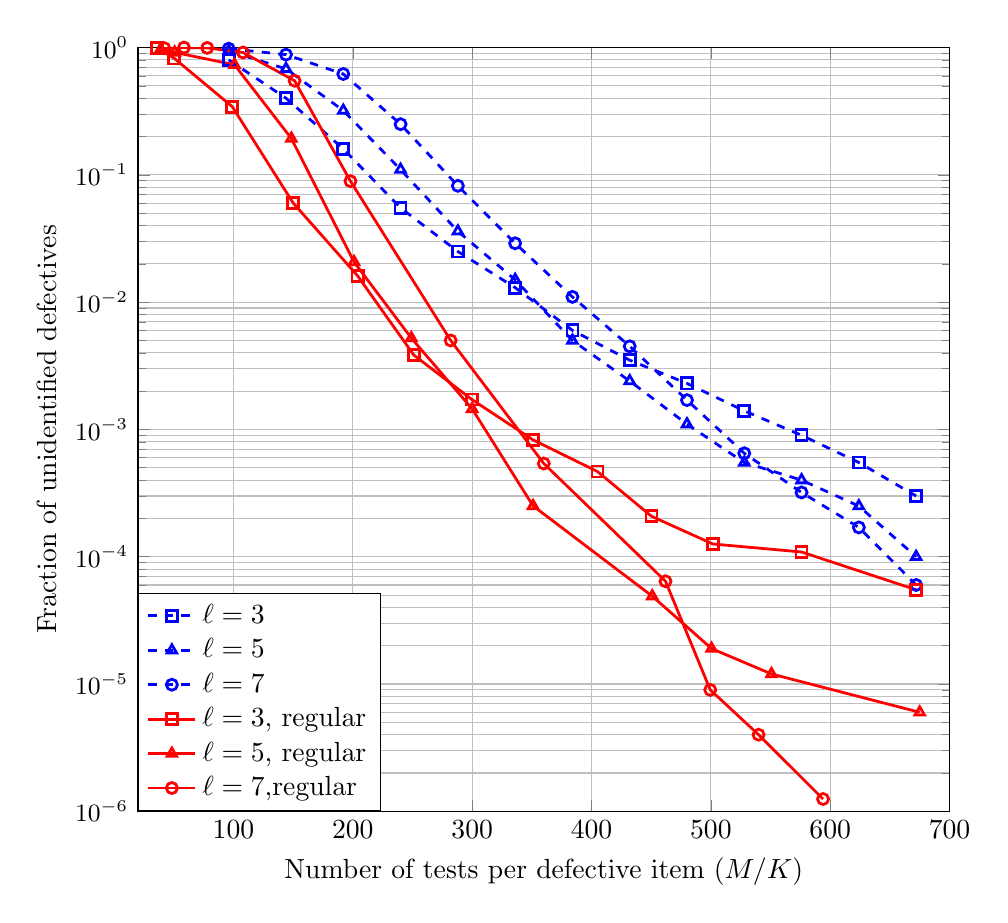
\begin{tikzpicture}
\def\fsize{\normalsize}
\pgfplotsset{every y tick label/.append style={font=\footnotesize}}
\pgfplotsset{every y tick label/.append style={font=\small}}

\begin{axis}[%
width=0.85\columnwidth,
height=0.8\columnwidth,
scale only axis,
xmin=20,
xmax=700,
xtick = {100,200,...,700},
xmajorgrids,
ymode=log,
ymin=1e-06,
ymax=1,
yminorticks=true,
ymajorgrids,
yminorgrids,
xlabel={\fsize{Number of tests per defective item ($M/K$)}},
ylabel={\fsize{Fraction of unidentified defectives}},
legend style={at={(0,0)},anchor=south west,draw=black,fill=white,legend cell align=left,font=\fsize}
]
\addplot [color=blue,dashed, mark=square,mark options={solid},line width=1pt]
  table[row sep=crcr]{96	0.8\\
144	0.4\\
192	0.16\\
240	0.055\\
288	0.025\\
336	0.013\\
384	0.006\\
432	0.0035\\
480	0.0023\\
528	0.0014\\
576	0.0009\\
624	0.00055\\
672	0.0003\\
};
\addlegendentry{$\ell=3$};

\addplot [color=blue,dashed,line width=1pt,mark=triangle,mark options={solid}]
  table[row sep=crcr]{96	0.94\\
144	0.68\\
192	0.32\\
240	0.11\\
288	0.036\\
336	0.015\\
384	0.005\\
432	0.0024\\
480	0.0011\\
528	0.00055\\
576	0.0004\\
624	0.00025\\
672	0.0001\\
};
\addlegendentry{$\ell=5$};


\addplot [color=blue,dashed,mark=o,mark options={solid},line width=1pt]
  table[row sep=crcr]{96	0.98\\
144	0.88\\
192	0.62\\
240	0.25\\
288	0.082\\
336	0.029\\
384	0.011\\
432	0.0045\\
480	0.0017\\
528	0.00065\\
576	0.00032\\
624	0.00017\\
672	6e-05\\
};
\addlegendentry{$\ell=7$};

%\addplot [color=blue,dashed,line width=3pt,mark=square,mark options={solid}]
%  table[row sep=crcr]{96	0.98\\
%144	0.94\\
%192	0.85\\
%240	0.52\\
%288	0.21\\
%336	0.065\\
%384	0.024\\
%432	0.0095\\
%480	0.0032\\
%528	0.0014\\
%576	0.00055\\
%624	0.00024\\
%672	0.0002\\
%};
%\addlegendentry{$l=9$};

\addplot [color=red,solid, line width=1pt, mark=square,mark options={solid}]
  table[row sep=crcr]{
36  0.99261\\
50.40      8.22e-1 \\
99.00      3.43e-1\\
150.00    6.01e-2 \\
204.00    1.61e-2\\
251.10    3.84e-3 \\
299.70    1.72e-3  \\
 351.00    8.28e-4 \\ 
 405.00    4.67e-4\\
 450.24    2.08e-4\\
 501.60  1.26e-4 \\  
 576.00  1.09e-4\\
672.00   5.50e-5\\
%66  0.80679\\
%79.20  0.65094\\
%99  0.4133 \\
%120     0.1596\\
%150     0.06312\\
%180 0.02797\\ 
%210     0.01396\\
%253.8  0.00344 \\
%307.8  0.00153\\
%324     0.00124 \\
%361.8  0.00078 \\
%369.6  0.00046 \\
%408     0.00031\\
%480.0  0.00021 \\
%672 0.000076\\
};
\addlegendentry{$\ell=3$, regular};

\addplot [color=red, solid, line width=1pt, mark=triangle,mark options={solid}]
  table[row sep=crcr]{
   39.000    0.970769\\
    50.700      9.16e-1   \\
100.800     7.33e-1   \\
148.500     1.93e-1   \\
201.000     2.07e-2  \\
249.000     5.22e-3  \\
300.000     1.450e-3\\
351.000     2.51e-4\\
%405.000     8.60e-5\\
450.900     4.90e-5\\
500.580     1.90e-5 \\
550.800     1.20e-5\\
%602.100 	  1.10e-5\\
675.000     6.00e-6\\
%   72.000    0.946226\\
% 132.000    0.327190\\
% 198.000    0.036304 \\
% 210.000    0.015015 \\
% 240.000    0.006573\\
% 270.000    0.003021\\
% 300.000    0.001460\\
% 360.000    0.000479\\
% 378.000    0.000157\\
% 453.600    0.000048\\
% 540.000    0.000013\\
% 604.800    0.000003\\
 };
\addlegendentry{$\ell=5$, regular};

\addplot [color=red, solid, line width=1.0pt,mark=o]
  table[row sep=crcr]{
42.00  0.99      \\
58.50	0.9995  \\
78.00    0.9937 \\
108.00   0.9142 \\
151.20  0.5487  \\
198.00 8.92e-2  \\
282.00  5.0e-3    \\
360.00  5.4e-4   \\
462.00  6.42e-5   \\
499.50  9.00e-6   \\
540.00  4.00e-6   \\
594.00  1.25e-6   \\
};
\addlegendentry{$\ell=7$,regular};

\end{axis}
\end{tikzpicture}%}
\end{frame}

%----------------------------------------------------------------------------------------------------------------------------------
\begin{frame}{Numerical results-Noisy GT}
\vspace{-1ex}
\begin{align*}
\vec{y}&=A\odot \vec{x} ~\oplus \vec{z}~~\quad	\text{where } z_i\sim \text{Ber}(q).
\end{align*}

\centering
\resizebox{0.6\textwidth}{!}{% This file was created by matlab2tikz v0.4.7 running on MATLAB 7.14.
% Copyright (c) 2008--2014, Nico Schlömer <nico.schloemer@gmail.com>
% All rights reserved.
% Minimal pgfplots version: 1.3
% 
% The latest updates can be retrieved from
%   http://www.mathworks.com/matlabcentral/fileexchange/22022-matlab2tikz
% where you can also make suggestions and rate matlab2tikz.
% 
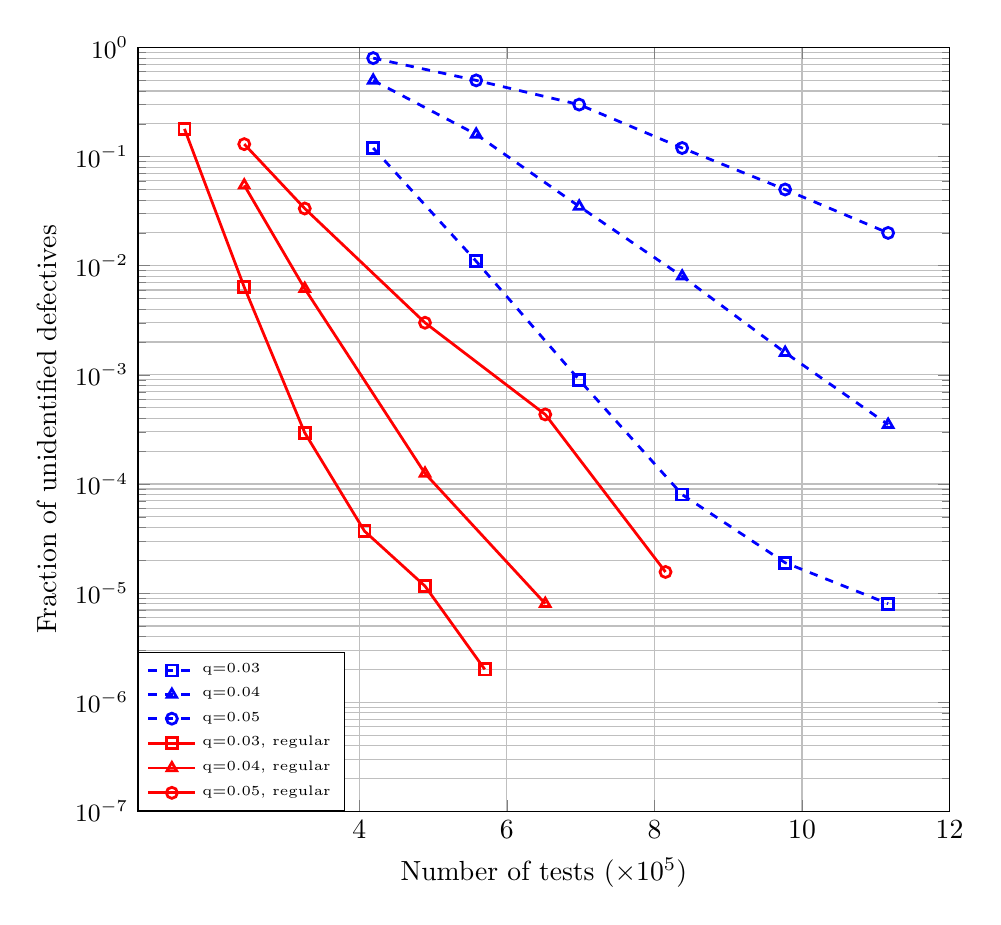
\begin{tikzpicture}
\def\fsize{\normalsize}
\pgfplotsset{every y tick label/.append style={font=\footnotesize}}
\pgfplotsset{every y tick label/.append style={font=\small}}

\begin{axis}[%
width=0.85\columnwidth,
height=0.8\columnwidth,
scale only axis,
xmin=1,
xmax=12,
xmajorgrids,
xtick = {4,6,8,10,12},
ymode=log,
ymin=1e-07,
ymax=1,
yminorticks=true,
ymajorgrids,
yminorgrids,
xlabel={\fsize{Number of tests ($\times 10^5$)}},
ylabel={\fsize{Fraction of unidentified defectives}},
legend style={at={(0,0)},anchor=south west,draw=black,fill=white,legend cell align=left, font=\tiny}
]
\addplot [color=blue,dashed,line width=1.0pt,mark=square,mark options={solid}]
  table[row sep=crcr]{4.1877504	 0.12\\
5.5836672	0.011\\
6.979584 	0.0009\\
8.3755008	8e-05\\
9.7714176	1.9e-05\\
11.1673344	 8e-06\\
};
\addlegendentry{q=0.03};

% pattern=on 1pt off 3pt on 3pt off 3pt
\addplot [color=blue,dashed,line width=1.0pt,mark=triangle,mark options={solid}]
  table[row sep=crcr]{4.1877504 	0.5\\
5.5836672		0.16\\
6.979584 		0.035\\
8.3755008		0.008\\
9.7714176	 	0.0016\\
11.1673344 	0.00035\\
};
\addlegendentry{q=0.04};

%\addplot [color=blue,dashed,line width=2.0pt,mark=asterisk,mark options={solid}]
\addplot [color=blue,dashed,line width=1.0pt,mark=o,mark options={solid}]
  table[row sep=crcr]{4.1877504 	0.8\\
5.5836672		0.5\\
6.979584 		0.3\\
8.3755008		0.12\\
9.7714176		0.05\\
11.1673344 	0.02\\
};
\addlegendentry{q=0.05};



\addplot [color=red,solid,line width=1.0pt,mark=square,mark options={solid}]
  table[row sep=crcr]{
 1.63     0.1797 \\
 2.44     6.363e-3\\
3.26     2.948e-4\\
4.07     3.700e-5\\
4.89     1.16e-5\\
5.70    2.00e-6\\
};
\addlegendentry{q=0.03, regular};


\addplot [color=red,solid,line width=1.0pt,mark=triangle,mark options={solid}]
  table[row sep=crcr]{
2.44     5.469e-2\\
3.26     6.168e-3\\
4.89     1.250e-4\\
6.52     8.000e-6\\
};
\addlegendentry{q=0.04, regular};

\addplot [color=red,solid,line width=1.0pt,mark=o,mark options={solid}]
  table[row sep=crcr]{
   2.44  	1.302e-1  \\
   3.26  	3.348e-2\\
   4.89	    3.005e-3\\
   6.52	    4.340e-4\\
   8.15     1.5625e-5  \\
};
\addlegendentry{q=0.05, regular};



\end{axis}
\end{tikzpicture}}
\end{frame}